\subsection{Zbiór "Wine"}
    \begin{figure}[H]
        \center
        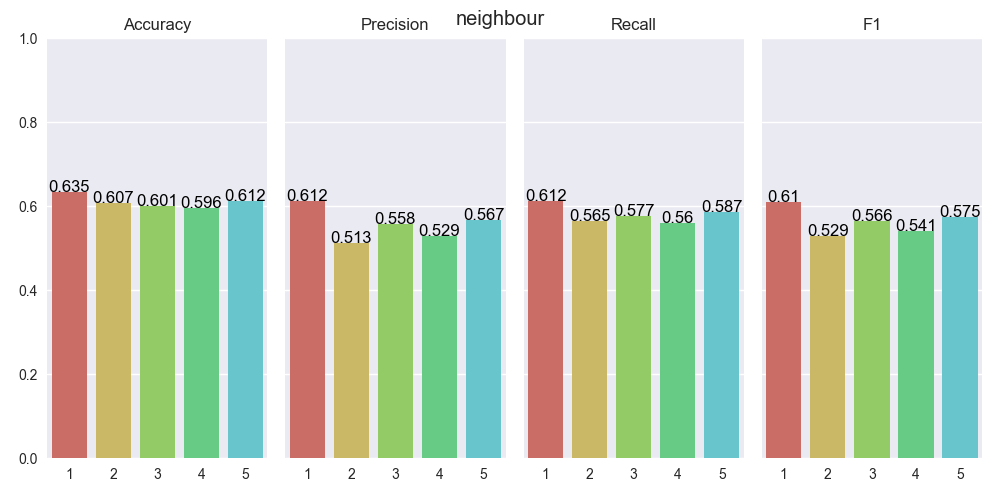
\includegraphics[width=\textwidth]{resources/plots/wine_KFold_neighbour.png}
        \caption{Wykres wartości miar dla zbioru "Wine" dla różnej liczby sąsiadów (kroswalidacja zwykła).}
    \end{figure}

    \begin{figure}[H]
        \center
        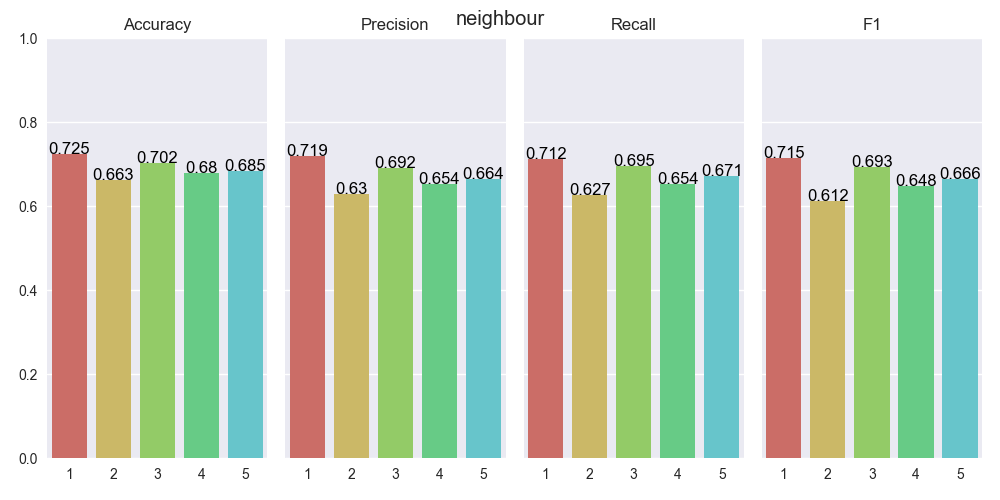
\includegraphics[width=\textwidth]{resources/plots/wine_StratifiedKFold_neighbour.png}
        \caption{Wykres wartości miar dla zbioru "Wine" dla różnej liczby sąsiadów (kroswalidacja stratyfikowana).}
    \end{figure}

    \pagebreak

    \begin{figure}[H]
        \center
        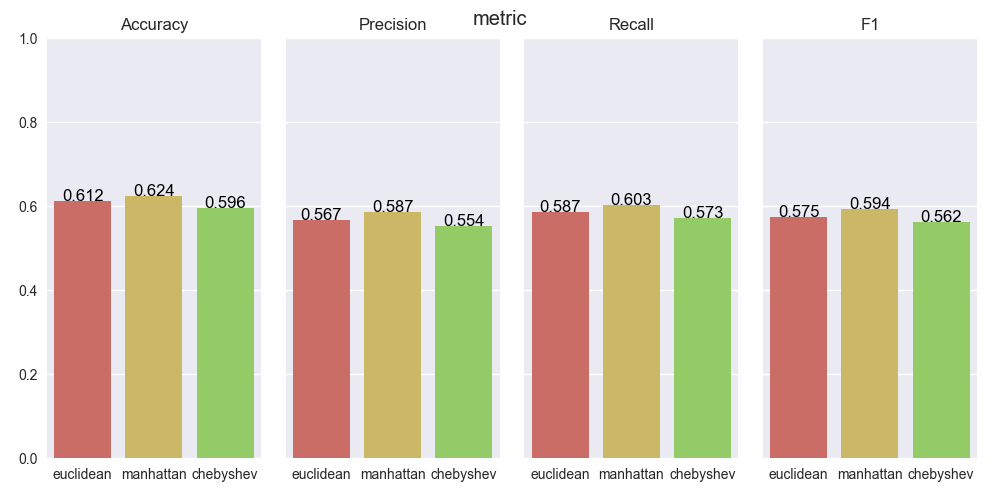
\includegraphics[width=\textwidth]{resources/plots/wine_KFold_metric.png}
        \caption{Wykres wartości miar dla zbioru "Wine" dla różnych metryk odległości (kroswalidacja zwykła).}
    \end{figure}

    \begin{figure}[H]
        \center
        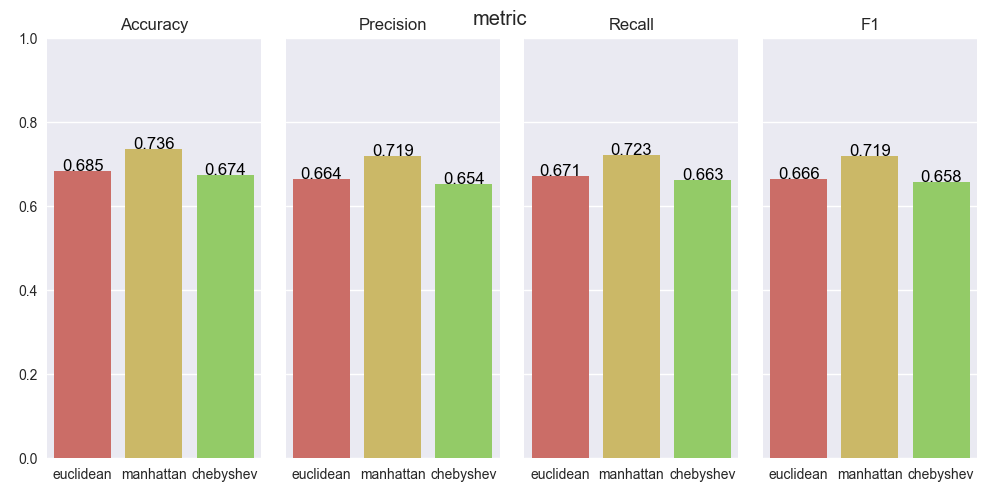
\includegraphics[width=\textwidth]{resources/plots/wine_StratifiedKFold_metric.png}
        \caption{Wykres wartości miar dla zbioru "Wine" dla różnych metryk odległości (kroswalidacja stratyfikowana).}
    \end{figure}

    \pagebreak

    \begin{figure}[H]
        \center
        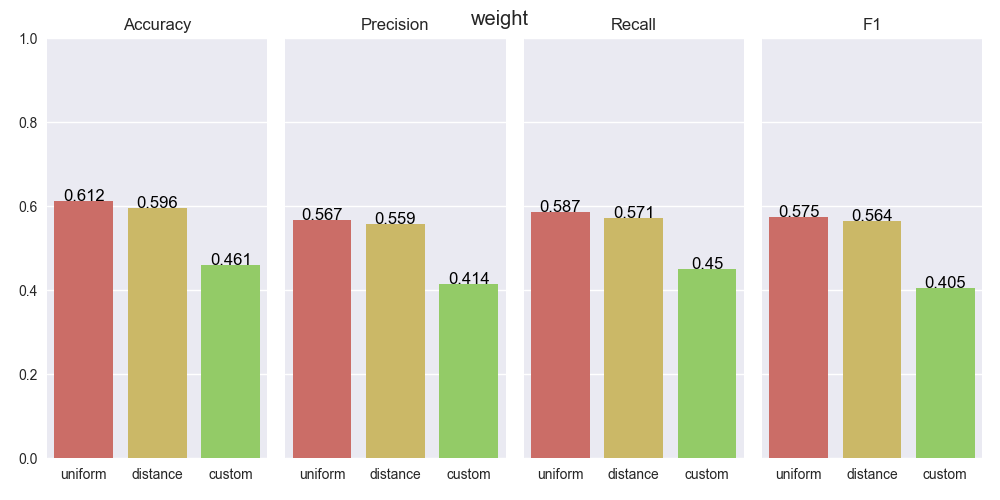
\includegraphics[width=\textwidth]{resources/plots/wine_KFold_weight.png}
        \caption{Wykres wartości miar dla zbioru "Wine" dla różnych sposobów głosowania (kroswalidacja zwykła).}
    \end{figure}

    \begin{figure}[H]
        \center
        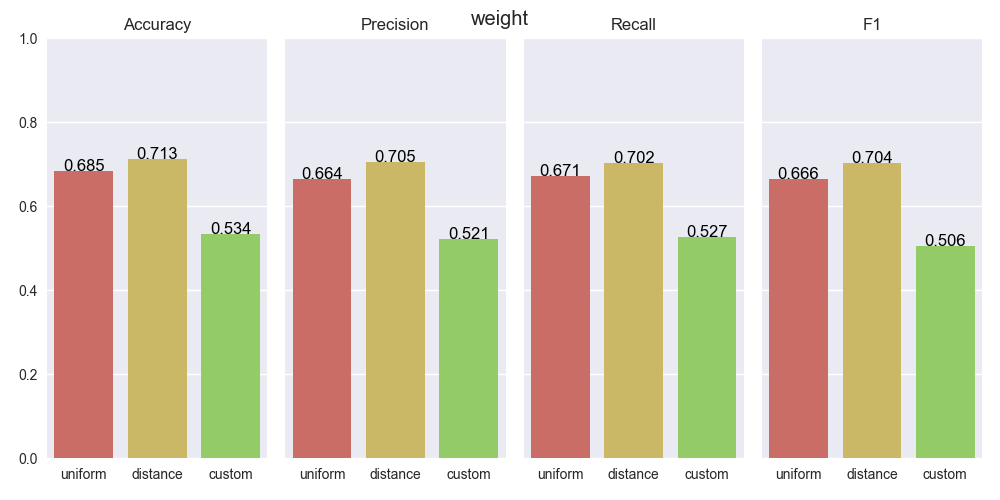
\includegraphics[width=\textwidth]{resources/plots/wine_StratifiedKFold_weight.png}
        \caption{Wykres wartości miar dla zbioru "Wine" dla różnych sposobów głosowania (kroswalidacja stratyfikowana).}
    \end{figure}


    \begin{figure}[H]
        \center
        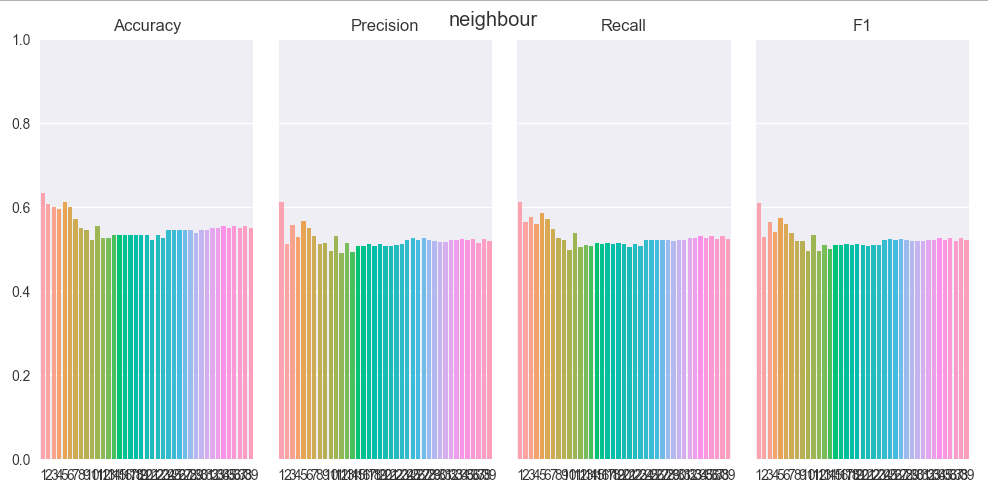
\includegraphics[width=\textwidth]{resources/plots/wine_nonnormalized_neighbours_kfold.png}
        \caption{Wykres wartości miar dla zbioru "Wine" dla większej liczby sąsiadów (kroswalidacja zwykła, dane nieznormalizowane).}
    \end{figure}

    \begin{figure}[H]
        \center
        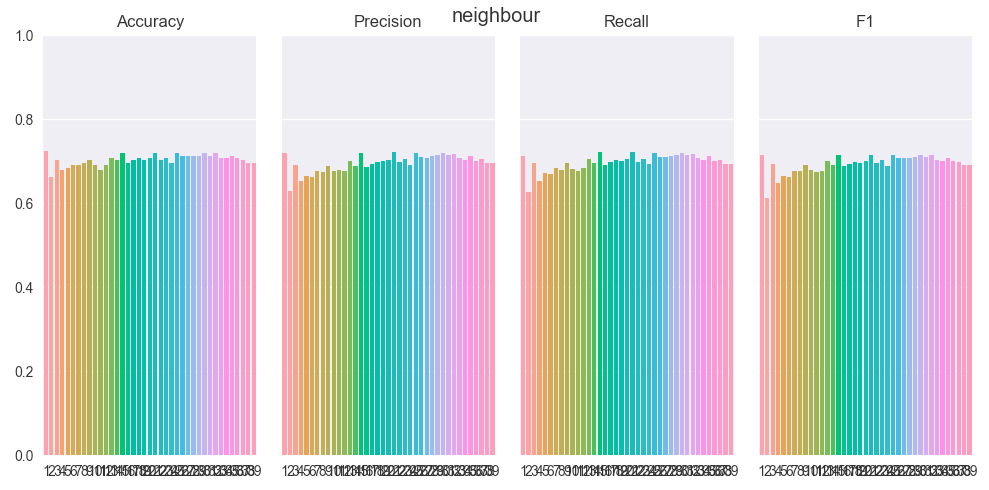
\includegraphics[width=\textwidth]{resources/plots/wine_normalized_neighbours_kfold.png}
        \caption{Wykres wartości miar dla zbioru "Wine" dla większej liczby sąsiadów (kroswalidacja zwykła, dane znormalizowane).}
    \end{figure}

    \begin{figure}[H]
        \center
        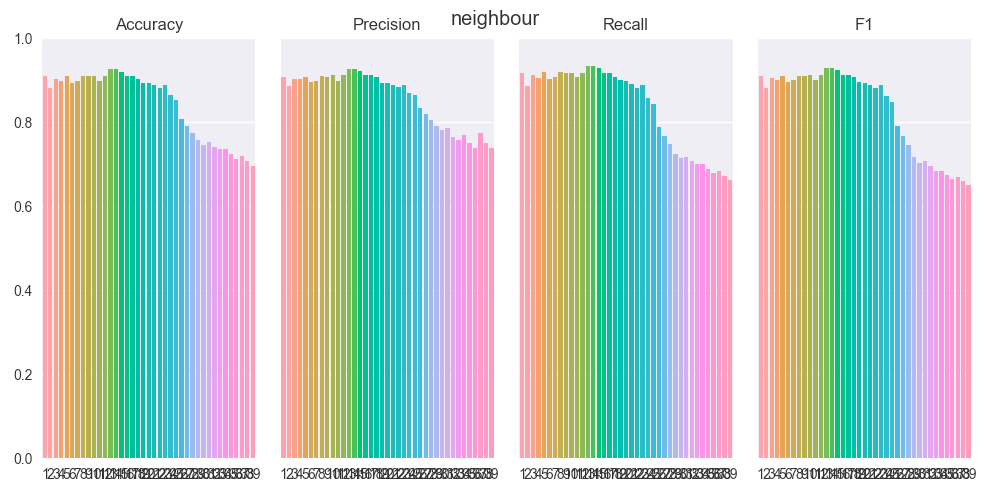
\includegraphics[width=\textwidth]{resources/plots/wine_nonnormalized_neighbours_skfold.png}
        \caption{Wykres wartości miar dla zbioru "Wine" dla większej liczby sąsiadów (kroswalidacja stratyfikowana, dane nieznormalizowane).}
    \end{figure}

    \begin{figure}[H]
        \center
        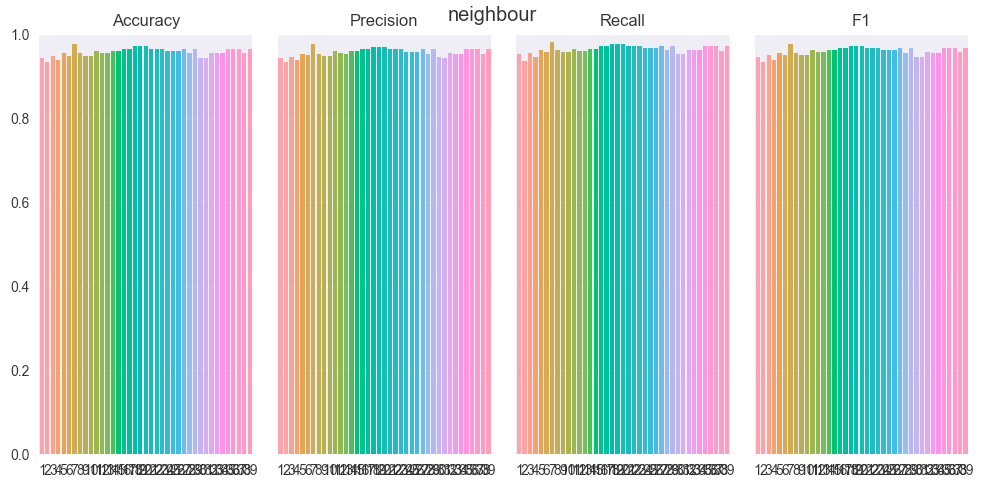
\includegraphics[width=\textwidth]{resources/plots/wine_normalized_neighbours_skfold.png}
        \caption{Wykres wartości miar dla zbioru "Wine" dla większej liczby sąsiadów (kroswalidacja stratyfikowana, dane znormalizowane).}
    \end{figure}